\documentclass[letterpaper, titlepage, freqn]{article}

\usepackage[utf8]{inputenc}
\usepackage[slovene]{babel}
\usepackage{amsmath}
\usepackage{amssymb}
\usepackage{graphicx}
%\usepackage{url}

\begin{document}
\title{Seminar \\ Kriptovalute}
\author{Lana Herman, Tjaša Renko, Eva Rozman \& Nejc Ševerkar \\ mentor Janez Bernik}
\date{\today}
\maketitle

\begin{abstract}
\begin{center}
V seminarski nalogi sta opisani in primerjani decentralizacija ter monetarna politika. Podrobno je razloženo delovanje kriptovalut (rudarjenje, tehnologija blockchain idr.), njihova zgodovina, razvoj in pomen ter primeri. Opisane so lastnosti in problemi Initial Coin Offering ter primerjava z bolj klasičnim IPO. Predstavljene so nekatere izmed najpomembnejših kriptovalut, Ripple, Ethereum in Bitcoin. Razložene so tudi možne zlorabe, povezane s kriptovalutami, posebej Ponzi shema in mrežni marketing.
\end{center}
\end{abstract}

\tableofcontents

\addtocontents{toc}{\setcounter{tocdepth}{3}}

\clearpage

\section{Ideologija decentralizacije}

Def: Decentralizacija je proces, kjer so dela organizacije, predvsem ta povezana s planiranjem in odločanjem, distributirana stran od centralne, avtoritetne skupine, med vse dele organizacije.

Moralno: Sistem je decentraliziran, ko so neke odločitve agentov izvršene brez centraliziranega nadzora ali procesiranja.

Opomba: Decentralizacija ne pomeni, da centra v sistemu ni, pomeni le da ima vsak uporabnik enake pravice glede razpolaganja in upravljanja tega sistema, kar še vedno dopušča naravno formacijo nekega centra (npr. večja skupina strežnikov v P2P sistemu).

Zgled: Abstraktna predstavitev centraliziranega in decentraliziranega sistema z grafi.\\

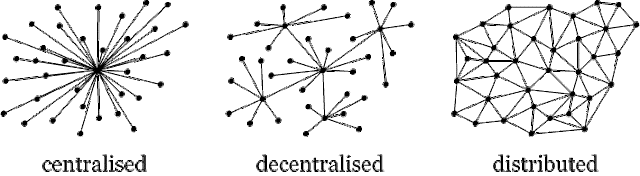
\includegraphics[height=3.5cm]{ponazoritev_decentralizacije}\\

Na grafih se vidi manjša povezanost uporabnikov pri centraliziranem sistemu, kot pri decentraliziranem, saj je pri centraliziranem delovanje odvisno le od centra sistema, pri decentraliziranem pa se formira več centrov, saj ima vsak uporabnik možnost prispevanja k drugim uporabnikom preko danega sistema.
Posledica koncentracije centraliziranega grafa v eni točki je odvisnost delovanja celotnega sistema od manjše (centralne) skupine, in ne od uporabnikov samih. 
Distributivnost se nanaša bolj na lokacijo delov sistema (če so deli sistema razpršeni (dosegljivi) med uporabnike, potem so distributirani) in je lahko nadgradnja tako decentraliziranega kot centraliziranega sistema (omenimo zaradi P2P sistema, na katerem sloni blockchain tehnologija).

Primera: Facebook je primer centraliziranega sistema, saj mora vsaka uporaba sistema iti preko določene skupine strežnikov, ki hranijo vse informacije o uporabnikih, ti pa enakih pravic, iz razlogov anonimnosti, ne morejo imeti.
Primer decentraliziranega sistema pa so torrent mreže, saj njihovo delovanje ni odvisno od enega centra, temveč uporabnikov, ki delijo podatke med sabo, kar močno vpliva na hitrost sistema.

Prepoznavanje centraliziranega sistema: V splošnem centralizacija sistema ni nujno očitna (npr. github). Sistem lahko prepoznamo kot centraliziran, če obstaja nek center sistema, ki ima več pravic glede upravljanja kot njegovi uporabniki.
Za zahtevnejše sisteme je za njihovo analitiko pametno uporabiti teorijo sistemov (ang. sistem theory).\\


\section{Monetarna politika}

\subsection{Ekonomska politika}

Ekonomska politika je organizirana akcija nosilcev (parlament, vlada, računsko sodišče, centralna banka), ki poskušajo s pomočjo instrumentov doseči najpomembnejše ekonomske cilje (gospodarski razvoj, stabilna rast cen, nizka stopnja nezaposlenosti, uravnoteženi odnosi s tujino). Deli se na fiskalno, monetarno in zunanje - trgovinsko politiko.\\

\subsection{Monetarna politika}

Monetarna politika je sistem ukrepov, ki jih izvaja in vodi centralna banka v državi z namenom doseganja ekonomskih ciljev. Monetarna politika predvsem določa količino denarja v obtoku.\\

\subsection{Funkcije in cilji centralne banke}

Glavni cilji centralne banke so ohranjanje stabilnosti cen, zviševanje zaposlenosti ter zagotavljanje zmerne dolgoročne obrestne mere.
Centralna banka izdaja primarni denar. Kreditira na tri načine, in sicer krediti državi (odkupuje državne obveznice, ki jih plača z novo izdanim primarnim denarjem), krediti tujini (uravnava devizni tečaj) ter krediti poslovnim bankam (centralna banka igra vlogo posojilodajalca v zadnji sili).
Instrumenti denarne politike so obrestna mera (če se poveča količina denarja v obtoku, se obrestne mere znižajo), obvezna rezerva, delovanje banke na odprtem trgu (nakup in prodaja vrednostnih papirjev - če CB kupi vrednostne papirje, imajo poslovne banke več denarja za multiplikacijo, če pa proda, imajo manj denarja), vloga posojilodajalca v skrajni sili (v skrajnem primeru lahko CB intervenira oz. rešuje neko situacijo).\\

\subsection{Bančni sistem}

Bančni sistem tvorijo centralna banka in poslovne banke, ki jih opredeljujemo kot depozitne finančne institucije. Skupna lastnost depozitnih finančnih institucij je zbiranje finančnih prihrankov z vlogami varčevalcev. Varčevalcem so na voljo različni računi, na katere vlagajo svoje prihranke ob različnih pogojih glede dospetja, možnosti dviga, donosnosti in drugih storitev. Prihranke, zbrane z vlogami, prenašajo takšne finančne institucije na investitorje, predvsem v obliki posojil. Štiri osnovne finančne oblike institucij so poslovne banke, hranilnice, kreditne zadruge in vzajemne hranilnice.
Centralna banka omogoča nemoteno funkcioniranje bančnega in finančnega sistema.
Med osnovne bančne funkcije štejemo zbiranje sredstev (področje depozitnega poslovanja in poslovanja z vrednostnimi papirji), usmerjanje sredstev (kreditiranje, garancijsko poslovanje, nakup vrednostnih papirjev), finančno dohodkovna funkcija (področje zakladništva), devizno poslovanje, itd.
Poslovne banke so organizirane izrazito hierarhično, s številnimi ravnmi odločanja, z natančno predpisanimi postopki, ki preprečujejo posameznim oddelkom ali zaposlenim prilagajanje potrebam komitentov (fizična oseba, za katero banka opravlja bančne posle).
Osnovna načela poslovanja bank so načelo likvidnosti (banka mora biti vselej sposobna izpolnjevati svoje dospele obveznosti), načelo varnosti (banka mora biti sigurna, da bodo njeni poslovni partnerji v dogovorjenem roku izvršili vse svoje obveznosti do banke), načelo rentabilnosti (banke usmerjajo svoja sredstva v dobičkonosne naložbe) in načelo tržnosti (delovanje banke je usmerjeno k optimalni zadovoljitvi potreb komitentov, ob doseganju čim bolj ugodnega finančnega rezultata – dobička).
Temeljni cilj in namen ustanavljanja bank je bil in je vsekakor ustvarjanje dobička. Banka zato želi visoke aktivne obresti in nizke pasivne obresti. Obrestna mera kot cena vpliva na povpraševanje in ponudbo denarne akumulacije. Pri aktivnih obrestnih merah bo povpraševanje po kreditih padlo, pri nizkih pasivnih obrestnih merah pa se bo zopet zmanjšala ponudba presežkov denarne akumulacije.\\

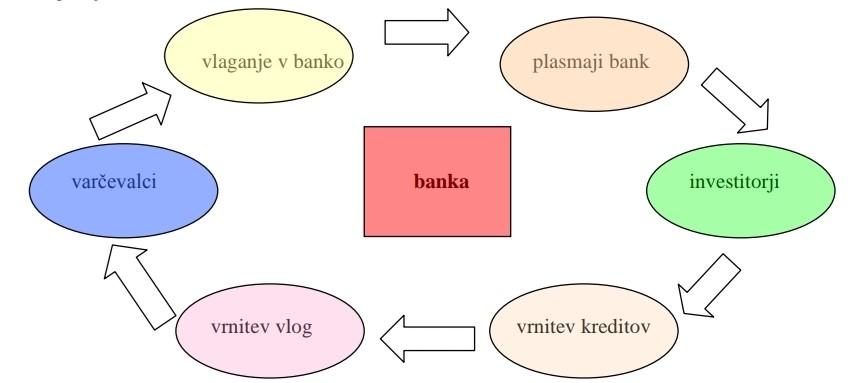
\includegraphics[height=5cm]{tokokrog_sredstev}\\

\subsection{Zgodovina monetarne politike}

Pred letom 1999 sta obstajali dve vrsti bank z dvema različnima pomenoma. To so bile investicijske banke in poslovne banke. Poslovne banke so imele nalogo, da dajejo posojila in sprejemajo depozite, tako da ponujajo tekoče in varčevalne račune. Investicijske banke pa so delovale samo na kapitalskih trgih. To so finančni trgi za kupovanje in prodajo dolgoročnih dolžniških ali delniških vrednostnih papirjev.
Po letu 1999 so se banke lahko združile in izvajale obe funkciji. Na kapitalskih trgih banke sklepajo tvegane posle. Če veliko izgubijo, davkoplačevalci plačajo varščino in zaščitijo prihranke potrošnikov.
Prva ideja centralizirane banke se je pojavila takoj po ustanovitvi Amerike, leta 1776. Argument za je bil, da potrebujejo močno centralno silo, ki bi pomagala gospodarstvu in prinesla stabilnost novemu monetarnemu sistemu v državi ter zagotavljanje kreditov za zasebne in javne potrebe. Argument proti je bil, da bo centralna banka spodnesla demokracijo.\\

\subsection{Denar}

Denar je splošni menjalni ekvivalent in praktično sredstvo za lažjo izmenjavo blaga. V začetni fazi je vlogo denarja prevzelo blago, ki so ga vsi radi sprejeli (npr. platno, školjke, koža, …). Zaradi ugodnih tehničnih lastnosti so vlogo denarja sčasoma prevzele plemenite kovine (zlato in srebro). Zaradi povečane proizvodnje blaga in storitev je začelo primanjkovati zlata za menjavo, zato smo zlato valuto zamenjali za papirno.
Funkcije denarja:
Menjalni posrednik - Denar omogoča lažjo menjavo blaga, storitev.
Plačilno sredstvo - Uporabljamo ga, ko svoje dolgove, ki jih bomo poravnali v prihodnosti izrazimo v denarju (npr. kredit, položnice, kazni, …).
Splošno merilo vrednosti - Z denarjem merimo vrednosti. V denarju izražena vrednost blaga je cena blaga.
Hranilec vrednosti - Denar se ne “pokvari” in ga lahko hranimo dolgo časa. To funkcijo opravljajo tudi delnice, obveznice in druge naložbe. Vendar pa je razlika v tem, da edino z denarjem lahko opravimo nakup takoj, vse ostale naložbe moramo najprej spremeniti v denar.
Kriptovalute lahko opravljajo funkcije menjalnega posrednika, plačilnega sredstva ter hranilca vrednosti. Kriptovalute so dostopne preko menjalnic, bitcoin bankomatov, pri nas tudi na bencinskih servisih in sedaj preko spleta. Tudi preko plačilnih kartic (Visa, Mastercard) je vkorakal v vsakdanji svet, saj lahko s tako kartico plačujemo blago in storitve kjerkoli obstaja bančni bankomat, ali POS terminal. Zato lahko kriptovalute opravljajo funkcijo plačilnega sredstva. V realni ekonomiji, pri izmenjavi blaga ali storitev med podjetji in državami, se Bitcoin dejansko redko uporablja in sicer zaradi volatilnosti, dolgih potrditvenih časov transakcij in uporabnikom še vedno tuje uporabe te tehnologije, čeprav lahko z mobilnim telefonom in elektronsko denarnico popolnoma nadomestimo plačilni promet preko bank.
Kriptovalute nekateri ljudi danes uporablja kot alternativo zlatu, torej kot hranilca vrednosti. Oba imata namreč nekaj podobnih lastnosti: produkcija je omejena in nista pod nadzorom držav. S to razliko, da so kriptovalute lažje prenosljive in bolj dostopne kot zlato. Če je Bitcoin sinonim za to, je Xaurum dejanski hranilec vrednosti. Ima podlago v fizičnem zlatu, ki ob novih vplačilih poskrbi, da fizična količina zlata vedno narašča.\\

\subsection{Zanimivosti}

 Dolar je v obdobju stotih let izgubil več kot 95 \% svoje kupne moči. Ker je nizka stopnja inflacije potrebna za dobro gospodarstvo, bo ta vrednost še naprej padala. Obstaja možnost, da dolar povsem izgubi svojo vrednost. To se s kriptovalutami ne more zgoditi, saj ni neke centralne sile, ki bi uravnavala vrednost kriptovalut. Zato bi lahko kriptovalute nadomestile papirno valuto.
Nobelov nagrajenec F. A. Hayek razlaga, da nobena centralna organizacija, ne glede na to, kako inteligentna se zdi, ne more vedeti vseh informacij, ki so potrebne v nekem gospodarstvu, da bi vedela, kakšne bi dejansko morale biti cene. Prava cena bi morala biti tista, ki jo zahteva trg po zakonih ponudbe in povpraševanja. Ko oseba, skupina ali organizacija poskušajo nadzorovati cene in ne delujejo skladno z zakoni o ponudbi in povpraševanju, izkrivljajo trg in ustvarjajo umetno pomanjkanje in presežek. Prave cene so, ko podjetja lahko neovirano določajo svoje cene na osnovi ponudbe in povpraševanja. Ko centralne banke določijo obrestne mere, uporabljajo nadzor nad cenami in izkrivljajo trg ter nanj pošiljajo nejasne cenovne znake.
S krajo kupne moči državljanov oz. zaradi inflacije centralne banke državljanom onemogočajo kopičiti bogastvo. Inflacija ne pospešuje ali spodbuja gospodarstva, ampak ustvarja iluzijo s povečanjem nominalnih številk namesto realnega števila gospodarske blaginje, uničuje valuto države. Inflacija je varljiva in povzroča utvare o veličastnosti bogastva in znanja. Nekateri služijo z inflacijo. Po ameriški revolucijski vojni so bile ustvarjene centralne banke. To je čas, ko inflacija doseže vrhunec. Z oslabitvijo dolarja vlada goljufa vojake in izvajalce tako, da jih plača v šibkejših dolarjih.\\

\subsection{Slabosti centralne banke}

John Maynard Keynes je v svoji knjigi Gospodarske posledice miru pisal, da je najboljši način za uničenje kapitalističnega sistema izkrivljanje valute. Vlada lahko z nenehnim procesom inflacije zasega, na skrivaj in neopazno, pomemben del bogastva svojih državljanov. Ni bolj subtilnega, bolj  gotovega načina za spreobrnitev obstoječih družbenih temeljev, kot je izkrivljanje valute. Proces vključuje vse skrite sile ekonomskih pravil na strani uničenja in to počne na način, da niti eden izmed milijona ljudi tega ne more diagnosticirati.
Ron Paul v svoji knjigi Ukinite zvezne rezerve piše, da bi ljudje brez zvezne rezerve uživali vse privilegije življenja modernega gospodarstva brez pomanjkljivosti poslovnih ciklov, mehurčkov, inflacije, netrajnostnih trgovinskih neravnovesij in eksplozivne rasti vlade, ki so jo pospešile zvezne rezerve.
Rešitev takšnega problema bi lahko bil sistem kriptovalut. Decentraliziran sistem.\\

\section{Kriptovalute}

\subsection{Zgodovina kriptovalut}

Prva digitalna valuta, imenovana echash, je bila teoritizirana leta 1983 in implementirana 1995 pod imenom Digicash. Omogočala je sicer anonimnost transakcij, a ni bila primer decentralizirane valute.
Prva decentralizirana kriptovaluta, BitCoin, je nastala leta 2009. Uporabljala je blockchain tehnologijo, ki je rešila veliko problemov prejšnjih neuspešnih kriptovalut (double spending) in omogočala močno stabilnost decentraliziranega sistema. Blockchain tehnologija bistveno prispeva  k funcionalnosti bitcoin sistema, torej si jo bomo podrobno ogledali in posušali razumeti njegovo delovanje.\\

\subsection{Podrobno o bitcoinovem delovanju}

Slovar:\\
Veriga blokov - blockchain\\
Polna vozlišča - full nodes\\
Lahka vozlišča - lightweight nodes\\
 
\subsubsection{Potrebne definicije}
 
SHA-256 (Secure Hash Algorithm) funkcija:\\
Funkcija, ki kot argument sprejme nek podatek in vrne 64 mestno kombinacijo alfa-numeričnih znakov, ki so za argument (skoraj) unikatni. Iz podpisa je (skoraj) nemogoče rekonstruirati vhoden podatek brez ustreznega ključa.\\

Hashcash sistem:\\
Sistem dokazila dela, ki ga uporablja bitcoin. Sistem sprejme podatek za validen, le če se njegova sha256 vrednost začne z 20-imi zaporednimi ničlami. To ponavadi zahteva veliko računalniške moči in veliko časa.\\
 
 
P = NP\\
P problemi so tisti, za katere je rešitev lahko preveriti in lahko posikati. NP polni problemi so tisti za katere je rešitev lahko preveriti, za iskanje te rešitve pa ni poznanega učinkovitega postopka, torej takšnega, ki bi porabil $O(n^{c})$ za nek c iz N časa. P = NP trditev trdi, da za vsak problem, katerega rešitev lahko hitro preverimo, obstaja postopek, ki takšno rešitev hitro najde.\\
 
\subsubsection{Koncept verige in blokov}

Veriga, imenovana blockchain idejno predstavlja javni izkaz odobrenih transakcij uporabnikov. Sestavljena je iz zaporedja blokov, v katerih so te transakcije zapisane. V osnovi so ti podatki vse kar predstavlja verigo.\\
 
\subsubsection{Omrežje}

Veriga blokov je v bitcoinovem sistemu oglaševana vsem uporabnikom na omrežju. Vedeti moramo, da ima vsak uporabnik dostop do te verige in jo lahko hrani na svojem računalniku in oglašuje po načelu P2P sistema z drugimi uporabniki.\\
 
\subsubsection{Klasifikacija Uporabnikov}

Obstajajo tri vrste uporabnikov sistema. Našteli jih bomo naraščajoče po funkcijah, torej bo vsak naslednje našteti uporabnik opravljal vse funkcije prejšnjih uporabnikov skupaj še z nekaterimi dodatnimi.
Prva vrsta so navadni uporabniki. Ti k sistemu prispevajo le z uporabo valute, torej trošijo, služijo in izmenjavajo. Ti niso zelo zanimivi.
Druga vrsta so vozlišča. To so uporabniki valute, ki hranijo verigo blokov na svojem računalniškem sistemu, jo posodabljajo in odobravajo transakcije uporabnikov (delijo se na polna in lahka vozlišča, katerih razlika je le delež hranjene verige).
Tretja vrsta so rudarji. To so polna vozlišča, ponavadi z večjo računalniško močjo, katero uporabljajo v namene ustvarjanja novih blokov v verigi in izbiranja odobrenih transakcij, ki bodo vključene v tega. Rudarji so najpomembnejši del sistema in podrobneje bomo njihovo vlogo v sistemu razumeli kasnje, za namen razumevanja prihodnje razlage.\\
 
\subsubsection{Sestava posameznega bloka v verigi}

Blok je sestavljen iz treh glavnih podatkovnih delov.
Prvi del so transakcije, odobrene preko sistema vozlišč in dane v blok preko rudarja, odgovornega za blokov nastanek. To so samo podatki o pošiljatelju, naslovniku in znesku prenesene valute.
Drugi del je sha256 vrednost prejšnjega bloka v verigi, ki predstavlja njegov digitalni podpis. Tu se moramo zavedati, da je vsak blok le neka skupina podatkov, ki jih lahko podamo kot argument tej funkciji. Ta vrednost torej poskrbi, da so bloki res povezani v podatkovno verigo.
Tretji del pa je neko število, ki ga imenujemo nonce. To število igra pomembno vlogo, ki jo bomo predelali kasneje.\\
 
 
\subsubsection{Pomen števila nonce}

Tu bomo definirali pravilo verige, in sicer edini bloki sprejeti v verigo so tisti, katerih sha256 vrednost se začne z 20-imi zaporednimi ničlami (Hashcash sistem). Rudar torej z ustvarjenjem novega bloka poišče takšno vrednost nonce števila, da bo z njim blok ustrezal pogoju verige.\\
 
\subsubsection{Nespremenljivost verige (Immutability)}

Vemo že da je vstop v verigo dovoljen le blokom, ki vsebujejo odobrene transakcije. Zakaj pa prejšnjih blokom v verigi ni mogoče spremeniti transakcijskih podatkov? Za to poskrbita podatka nonce in digitalni podpis predhodnika v vsakem bloku. Recimo, da zlobni uporabnik spremeni podatek v nekem bloku. Ker je spremenil podatek v bloku se spremeni njegov digitalni podpis, zaradi tega pa blok ne ustreza več pogoju verige, hkrati pa naslednik tega bloka ne kaže več nanj saj ima ta shranjen digitalni podpis prejšnjega bloka. Če uporabnik želi, da sistem neopazno sprejme njegovo verigo, mora ta prvo zadostiti pogoju verige, torej imeti ustrezno število nonce. Recimo, da ga uporabnik najde. Če sistemu sedaj objavi svojo verigo, bo ta opazil, da je veriga krajša kot prejšnja, torej jo bo zavrnil. Če želi uporabnik verigo narediti daljšo, bo moral popraviti naslednji blok, tako da se bo podatek digitalnega podpisa predhodnika v njej ujemal z njegovim blokom. Če to naredi se bo podatek v naslednjem bloku spremenil in bo spet odpadel iz verige. Tako bo moral spet skleniti verigo in tako spremeniti vsak nadaljni blok v verigi, skupaj z njimi pa prirediti število nonce, za kar porabi veliko časa. Verige ne bo moral nikoli ujeti, saj cel sistem gradi nove bloke medtem, ko on sam popravlja prejšnje.\\
 
\subsubsection{Transakcije}

Vemo že da so transakcije zabeležene v bloku. Njihova velikost je omejena z 1MB, zaradi česar je tudi število transakcij v bloku omejeno. Oglejmo si potek plačevanja transakcijskih stroškov.
Uporabniki sistema lahko sami določijo transakcijski strošek, ki ga zabeležijo ob transakcije. Ta strošek pripada rudarju, ki vključi transakcijo v blok, katerega je ustvaril, torej čim višji strošek uporabnik plača, čim hitreje bo njegova transakcija odobrena, saj bodo rudarji v svoje bloke vstavljali transakcije, z dražjimi cenami, saj te ob narejenem bloku poberejo oni.
Tako se cena transakcije na trgu oblikuje sama.\\

\subsection{Sklep delovanja sistema}

Delovanje sistema je nastavljeno tako, da se vsa pravila določijo s strani uporabnikov na naraven in včasih tekmovalen način. Tako ne potrebujemo postavljanja zakonov, povezanih s kriptovaluto, kar je največja razlika tega, decentraliziranega sistema, in centraliziranega, ki ga predstavlja monetarna politika.\\

\subsection{Motivacija rudarjev}

Vprašali se bomo zakaj rudarji prispevajo tako ogromen del svoje računalniške moči, potrebne za dokaz dela. Seveda je na prvi pogled očitno, da je njihova motivacija količina kriptovalute izdane rudarju ob nastanku novega bloka, a pri valuti bitcoin cash se je zgodilo, da je bila njena izdana cena manjša kot cena vzdrževanja računalnika med iskanjem rešitve Hashcash naloge. Kljub temu se sistem ni podrl in rudarji so še vedno nadaljevali delo na blokih. Njihova motivacija torej ni bila denarna, saj so z rudarjenjem zapravljali denar. Kaj bi torej bila njihova motivacija? Dober razlog je to, da imajo ti rudarji v lasti veliko količino valute in so ozaveščeni upada vrednosti, ki bi ga povzročila odpoved sistema. Zakaj pa potem, ne bi izplačali valute? Razlog za to pa je verjetno, da verjamejo v idejo kriptovalute, in potenciala zaradi katerega bo vrednost njihovega deleža narasla. Sistem torej temelji na močnem zaupanju uporabnikov vanj, zaradi česar ga vzdržujejo tudi če so s tem na izgubi.\\

\subsection{Zlorabe kriptovalut}

Enostavne in včasih legalne zlorabe kriptovalut so postale tradicionalen razlog za njihovo družbeno neodobravanje. Pogledali si bomo tri primere, ki nam bodo prikazali bistvo nevarnosti uporabe kriptovalut.
Value Overflow Incident: Primer zlorabe sistema, v katerem je neznana oseba priredila transakcijo, tako da je vsebovala 92 milijard bitnih kovancev, nakazanih na dva računa. Koda za avtorizacijo transakcij napake ni pazila, ker ni preverjala pravilnosti transakcij števila kovancov, ki so prebili meje predstavljivih števil (numerični izraz). Sistem pa je to napako hitro opazil in razcepil verigo na dva dela. Kljub nadaljevanju grajenja novih blokov s strani nekaterih rudarjev na pokvarjenem bloku je večina rudarjev gradila popravljeno verigo. Posledično je bila stara veriga dominirana, nova verzija verige pa je postala uradna transakcijska zgodovina.
Vdori v sistem: Vdori v denarnice uporabnikov so pri kriptovalutah postali pogost pojav. Razlog za to je, da so sistemi, ki nadzorujejo račune teh uporabnikov, prilagojeni njihovem računalniškem znanju, kar ogroža uporabnike. Ti se morajo v primeru kraje zanašati nase bolj kot bi se pri centraliziranih valutah, na katere so navajeni.
Pranje denarja: Za pranje denarja kriptovalut pomagajo mešalci, darknet in druge kriptovalute. Mešalci so storitve, ki omogočajo premešanje bitcoinov pred nakazilom v drugo denarnico. Darknet je skrito omrežje, do katerega se lahko dostopa le s pomočjo posebnih brskalnikov (Tor - anonimni, brezplačni open-source brskalnik). Postopek se začne tako, da je kriptovaluta poslana iz clearnet (navadno omrežje) denarnice v eno od skritih denarnic, na darknet-u. Ko je shranjena v to denarnico, se uporabijo mešalniki. Ti bodo samodejno razdelili kriptovaluto na več naslovov, ki jih gostijo strežniki na darknet omrežju. Ko je končano, se kriptovaluta lahko trguje z drugimi kriptovalutami.
Pranje denarja je bilo med letoma 2013 in 2016 odgovorno za en odstotek vseh transakcij s kriptovaluto bitcoin. Pranje denarja preprečujejo s procesoma KYC (Know Your Customer) in AML (Anti Money Laundering).\\

\subsection{Value Overflow Incident}

Primer zlorabe sistema, v katerem je neznana oseba priredila transakcijo, tako da je vsebovala 92 milijard bitnih kovancev, nakazanih na dva računa. Koda za avtorizacijo transakcij napake ni pazila, ker ni preverjala pravilnosti transakcij števila kovancov, ki so prebili meje predstavljivih števil (numerični izraz). Sistem pa je to napako hitro opazil in razcepil verigo na dva dela. Kljub nadaljevanju grajenja novih blokov s strani nekaterih rudarjev na pokvarjenem bloku je večina rudarjev gradila popravljeno verigo. Posledično je bila stara veriga dominirana, nova verzija verige pa je postala uradna transakcijska zgodovina.

\subsection{Vdori v sistem}

Vdori v denarnice uporabnikov so pri kriptovalutah postali pogost pojav. Razlog za to je, da so sistemi, ki nadzorujejo račune teh uporabnikov, prilagojeni njihovem računalniškem znanju, kar ogroža uporabnike. Ti se morajo v primeru kraje zanašati nase bolj kot bi se pri centraliziranih valutah, na katere so navajeni.

\subsection{Pranje denarja}

Za pranje denarja kriptovalut pomagajo mešalci, darknet in druge kriptovalute. Mešalci so storitve, ki omogočajo premešanje bitcoinov pred nakazilom v drugo denarnico. Darknet je skrito omrežje, do katerega se lahko dostopa le s pomočjo posebnih brskalnikov (Tor - anonimni, brezplačni open-source brskalnik). Postopek se začne tako, da je kriptovaluta poslana iz clearnet (navadno omrežje) denarnice v eno od skritih denarnic, na darknet-u. Ko je shranjena v to denarnico, se uporabijo mešalniki. Ti bodo samodejno razdelili kriptovaluto na več naslovov, ki jih gostijo strežniki na darknet omrežju. Ko je končano, se kriptovaluta lahko trguje z drugimi kriptovalutami.
Pranje denarja je bilo med letoma 2013 in 2016 odgovorno za en odstotek vseh transakcij s kriptovaluto bitcoin. Pranje denarja preprečujejo s procesoma KYC (Know Your Customer) in AML (Anti Money Laundering).\\

\subsection{Bitcoin in centralno bančništvo}

Negativen učinek centralnega bančništva je uničujoča inflacija za valuto, zmanjšanje kupne moči in s tem življenjskega standarda državljanov, prelaganje računa na poznejše generacije in drugi gospodarski problemi.
Zvezna vlada prihaja do točke, ko ne gre le za odklanjanje bitcoina, temveč se dejansko boji bitcoina in se mu na vso moč upira. Urad za finančno zaščito potrošnikov izdaja opozorila o tveganjih, povezanih z bitcoinom, da bi pomagal opozoriti in prestrašiti ljudi pred kriptovalutami.
Zvezne rezerve bodo potrebovale čas, da bodo ukinjene. Prvi korak v tem procesu se je že zgodil. Ljudje so začeli dvomiti vanje in njihovo vlogo v gospodarstvu. Drugi korak je, da se najde morebitna zamenjava, kar se trenutno izvaja. Trg sam je ponudil zamenjavo zveznih rezerv: bitcoin. Tretji korak je počasen proces zamenjave in sčasoma razpustitve zveznih rezerv potem, ko bo jasno, kako so alternative (bitcoin) učinkovitejše in izbrane na trgu kot prednostna možnost.\\

\subsection{ Zanimivosti}

Hibridna kriptovaluta je valuta, ki združi koncepta centralizacije in decentralizacije v mešano obliko, ki izkoristi prednosti obeh konceptov (implementacija v DasCoin kriptovaluti)
Najmanjša možna količina bitcoina je $10^{-6}$ bitcoina in je imenovana Satoshi, po anonimnemu izumitelju bitcoina, znanim pod psevdonimom Satoshi Nakamoto.
Kvantumni računalnik je nova vrsta računalnika, katerega hitrost bo eksponentno hitrejša od teh, ki jih imamo danes. Strokovnjaki sklepajo, da bo naznanitev obstoja takšnega računalnika nastopila kot izrudarjene celotne količine preostalega bitcoina, saj bodo naloge, potrebne za zrudarjenje novega bloka, zanj zanemarljivo lahke.\\

\subsection{Statistični podatki}

Dnevni obseg trgovanja z najbolj prepoznavno kriptovaluto bitcoin v zadnjih 24 urah je znašal 15,717,608,193 USD (8.5.2019 - CoinMarketCap) in tržno kapitalizacijo 104,556,636,036 USD (8.5.2019 - CoinMarketCap).
Letno naj bi tehnologija blokov banke spravila ob 65-80 milijard dolarjev zaslužka (WEF).
Kriptovalute predstavljajo konkurenco in nevarnost bančnemu sektorju, zaradi česar se bančni sektor intenzivno usmerja tudi v kripto svet, kar potrjuje tudi nakup kripto borze Polonix s strani banke Goldman Sachs (ameriška multinacionalna banka, skupno premoženje US\$933 billion (2018) - Wikipedia).
Španski bančni koncern Santander je celo trdil, da bo do leta 2022 tehnologija blockchain v bančni industriji lahko prihranila do 20 milijard dolarjev na leto.
V današnjem bančnem sistemu lahko izvedba mednarodnih plačil traja nekaj dni, da finančna sredstva dosežejo svoje cilje, poleg tega pa so lahko postopki dragi. S pomočjo tehnologije blockchain se lahko te vrste plačil takoj ali v nekaj minutah prenesejo z minimalnimi stroški transakcij (Pilkington 2015). \\

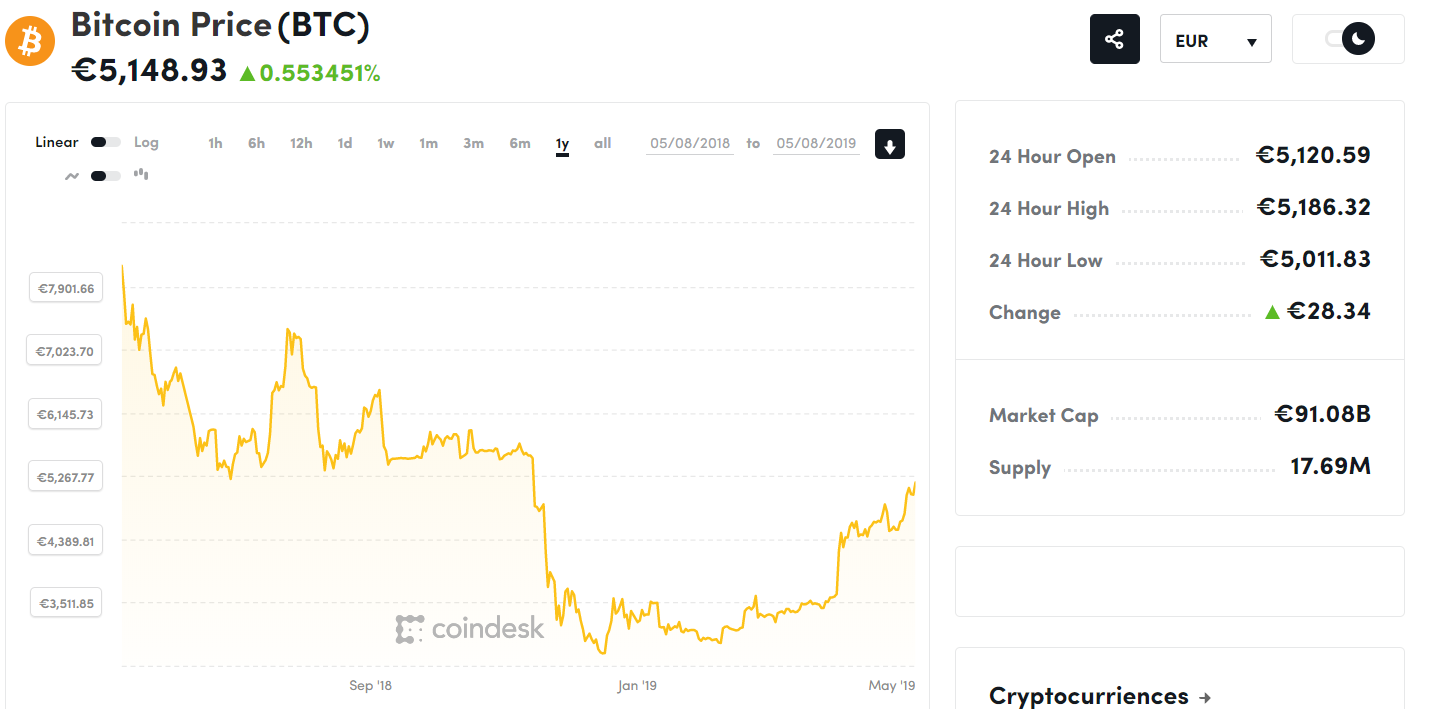
\includegraphics[height=6cm]{stat}\\

\subsection{Bitcoin in centralno bančništvo}

Negativen učinek centralnega bančništva je uničujoča inflacija za valuto, zmanjšanje kupne moči in s tem življenjskega standarda državljanov, prelaganje računa na poznejše generacije in drugi gospodarski problemi.
Zvezna vlada prihaja do točke, ko ne gre le za odklanjanje bitcoina, temveč se dejansko boji bitcoina in se mu na vso moč upira. Urad za finančno zaščito potrošnikov izdaja opozorila o tveganjih, povezanih z bitcoinom, da bi pomagal opozoriti in prestrašiti ljudi pred kriptovalutami.
Zvezne rezerve bodo potrebovale čas, da bodo ukinjene. Prvi korak v tem procesu se je že zgodil. Ljudje so začeli dvomiti vanje in njihovo vlogo v gospodarstvu. Drugi korak je, da se najde morebitna zamenjava, kar se trenutno izvaja. Trg sam je ponudil zamenjavo zveznih rezerv: bitcoin. Tretji korak je počasen proces zamenjave in sčasoma razpustitve zveznih rezerv potem, ko bo jasno, kako so alternative (bitcoin) učinkovitejše in izbrane na trgu kot prednostna možnost.\\

\section{Initial Coin Offering (ICO)}

\subsection{ Kaj je to}

Initial Coin Offering je način pridobivanja sredstev s strani podjetja z ustvarjanjem kriptovalute, ki jo lahko investitorji kupijo, običajno s klasičnim denarjem ali bitcoinom, v upanju, da bo pridobila na vrednosti, in s tem financirajo podjetje. To je praktično za startup podjetja, ki lahko tako dobijo sredstva, ne da bi se odpovedala deležu podjetja (glej IPO) ali se zadolžila, a tovrstni projekti niso omejeni samo na mlada podjetja. Kovanci, ki so najpogosteje izdani v projektu ICO, se imenujejo “utility tokens”. Predstavljajo obračunsko enoto omrežja. Njihovo število je fiksirano, zato je njihova vrednost odvisna od velikosti omrežja in količine transakcij. Včasih lastništvo nad kovanci iz ICO projekta pomeni tudi dostop do produkta ali storitve podjetja, redko predstavljajo celo volilno moč v podjetju. Obstajajo pa tudi kovanci s fiksno ceno in fiksnim številom ali s fiksno ceno in spreminjajočim številom . Slednji so prišli v uporabo šele pred kratkim.\\

\subsection{Kako poteka}

ICO je relativno malo reguliran. Ponekod je prepovedan, v večini držav pa dovoljen z malo omejitvami, včasih celo obdavčen. V Združenih državah Amerike in Evropski uniji mora ustrezati AML (Anti Money Laundering) in KYC (Know Your Customer) standardom, kar v grobem pomeni identifikacijo strank, sicer pa imajo njegovi ustvarjalci veliko svobode. Običajno je na začetku ustvarjen tako imenovani whitepaper, kar je dokument, v katerem je zapisano, koliko kovancev je ustvarjenih, kako dolgo bo trajal projekt (koliko časa bodo kovanci v prodaji) in kakšen delež bo podjetje zadržalo zase, kakšen je namen porabe pridobljenih sredstev, kdo so ustvarjalci projekta ter kakšen je podroben načrt projekta. Če projekt ne zbere dovolj sredstev v določenem času, se ta že zbrana vrnejo vlagateljem.\\

\subsection{Lastnosti}

Za ICO velja, da je investiranje dostopno javnosti in postopek hiter.  ICO je načeloma decentraliziran, saj ena sama oseba oziroma manjša skupina ljudi nima nadzora nad vrednostjo kovanca.\\

\subsection{Problemi ICO}

Stopnja tveganja je visoka, saj je uspeh projekta relativno malo verjeten, zaradi slabe regulacije pa so možne tudi prevare. Ena izmed težav ICO, ki pripomore k tveganju, je, da mora biti povpraševanje po kovancih večje od njihove inflacije, sicer projekt postaja podoben piramidni shemi. Piramidna oziroma Ponzijeva shema je model, pri katerem tisti kasneje vključeni financirajo prej vključene, dokler se sistem ne zruši zaradi pomanjkanja članov, ki bi morali dovesti denar za tiste na dnu piramide. Naslednji problem je, da sredstva vlagateljev pogosto financirajo nek koncept, ne že delujoče proizvodnje. Če produkt ali storitev, ki si jo podjetje prizadeva ustvariti, ne uspe, ima to slab učinek na vrednost njihovega kovanca. Poleg tega ljudje na začetku vlagajo denar in umetno napihnejo vrednost kovanca, ki potem strmo pade, če projekt ne uspe po pričakovanjih. Problem številnih kovancev je tudi, da so ustvarjeni le kot likvidnostno sredstvo in lahko podjetje deluje brez njih.\\

\subsection{Lastnosti uspešnega ICO}

Da je ICO uspešen, bi moral kovanec pridobivati na vrednosti, ICO pa bi moral biti upravičen in donosen za podjetje. To lahko dosežemo na primer na naslednje načine:\\
1. Lastništvo kovanca omogoča bodisi dostop do produkta ali posebne ugodnosti\\
2. Lastništvo kovanca nam da volilne pravice v podjetju\\
3. Kovanec se znotraj projekta uporablja za nagrajevanje\\
4. Kovanec prinaša prihodke\\

\subsection{Primer: Ethereum}

Ethereum je z 18 milijoni ameriških dolarjev, zbranimi v dobrem mesecu dni leta 2014, eden najuspešnejših ICO projektov vseh časov. Njegov cilj je sestavljanje aplikacij za transakcije in nadzorovanje denarja. Kovanec tega projekta se imenuje Ether in je tako uveljavljen, da se zdaj poleg Bitcoina pogosto uporablja za nakup ostalih kovancev, ustvarjenih prek ICO. Prav tako kot Bitcoin temelji na tehnologiji blockchain in dokazilu o delu ter je tako popolnoma decentraliziran. Razloge za uspeh Ethereuma lahko najdemo v tako imenovanih pametnih oziroma kriptopogodbah, ki so v bistvu programi, ki nadzorujejo transakcije pod vnaprej določenimi pogoji, ter Enterprise Ethereum Alliance (EEA), ki kostumizira Ethereum za industrijska podjetja in ga s tem naredi privlačnega za finančno močne organizacije, pa tudi posamezniki si lahko prilagodijo pogodbe za svoje potrebe. Z vzponom EEA je postal Ethereum izjemno popularen na kitajskem in južnokorejskem trgu.\\

\subsection{Za primerjavo: Initial Public Offering (IPO)}

Initial Public Offering je prodajanje deleža podjetja javnosti (delničarji). Prav tako kot Initial Coin Offering je IPO način financiranja podjetja, a le s strani bank ali drugih velikih, akreditiranih investitorjev. Postopek je dobro reguliran, torej so si različni IPO med sabo veliko bolj podobni. Regulacija podaljšuje tudi čas, ki ga investitor zapravi za vlaganje, pa tudi stroški projekta so višji kot pri ICO, predvsem zaradi bančnih provizij in pravnih stroškov. Podjetje mora tudi razkriti svoje finančno stanje in določene informacije o poslovanju. Investicija je tako manj tvegana zaradi skoraj ničelne možnosti prevar. IPO je centraliziran proces.\\

\subsection{Alternativno: Security Token Offering (STO)}

Security Token Offering je bolj podoben ICO, a s pomembnima razlikama. Tu investitor vedno kupi “security token”. To pomeni, da ima kovanec kritje v obliki lastniških pravic. Lastnik takega kovanca si lahko, odvisno od pogodbe, obeta prihodke iz premoženja ali prihodkov (dividende) podjetja, volilne pravice in podobno. Druga razlika je, da je STO bolj reguliran kot ICO. Vlagatelji so zaščiteni in projekt je transparenten, nadzorovan ter obdavčen. Sredstva, zbrana z STO, morajo biti porabljena tako, kot je bilo zagotovljeno v prej pripravljenem dokumentu. Zaradi tega in same definicije kovanca je vlaganje v tak projekt manj tvegano. STO ni več popolnoma decentraliziran.\\

\section{Ripple}

Ripple je mednarodna plačilna platforma z lastno valuto, imenovano XRP ali pogovorno Ripple. Nastala je leta 2012 in je logičen naslednik prvotno zasnovane infrastrukture globalnih plačil, PayPal, ki je nastala konec 20. stoletja in je za prenos potrebovala dneve. Ripple je izjemno hiter, za povprečno transakcijo porabi 3 sekunde. Banka lahko preko njega pošlje plačilo poljubni banki v tujini, omrežje pa nadzoruje transakcijo, računa njene stroške in pretvarja valute. Valuta se je pojavila šele kasneje, sistem je bil namreč najprej zasnovan le kot prostor za izvajanje transakcij ostalih klasičnih in kriptovalut. Ripple je poseben, ker ne uporablja dokaza o delu, temveč svojo različico tehnologije blockchain, v kateri ni vsak uporabnik strežnik, transakcije pa potrjujejo banke in druge finančne organizacije. Ta v resnici z današnjo definicijo te tehnologije nima veliko skupnega. Je centralizirana valuta, ki se je razvila med poskušanjem posodobitve svetovnega finančnega sistema namesto drastičnim spreminjanjem, kot se je Bitcoin. Zaradi tega je za banke bolj zanimiva. XRP izdajo Ripple Labs, ne morejo se rudariti in možno število enot v obtoku ni omejeno in jih je veliko več kot Bitcoinov. Kot platforma ima tudi kovanec glavni cilj biti uporabljan v mednarodnem bančnem sistemu. Vrednost XPR bi močno poskočila, če bi se začele banke odločati v smeri njegove uporabe kot lastne kriptovalute. Sedaj, ko ima nizko ceno (0,297106 USD 9. 5. 2019 zvečer), je po eni strani zanimiva investicija, po drugi pa je tako že nekaj let in nove valute se množijo, s tem pa možnost za uspeh pada. Po tržni kapitalizaciji je leta 2017 za kratek čas celo prevzela drugo mesto med kriptovalutami. Tržna kapitalizacija je število izdanih delnic, pomnoženo s tržno ceno delnice. Pomembna je, ker nam pove, da so investitorji zainteresirani. Naslednje leto je bilo podjetje toženo zaradi neregistrirane prodaje kovancev, in čeprav zmaga, izgubi veliko zaupanja investitorjev in vrednost strmo pade.\\

\section{Zlorabe kriptovalut}

\subsection{Mrežni marketing}

Mrežni marketing (multi-level marketing ali MLM) je poslovni model, pri katerem prihodek podjetja izhaja iz prodaje izdelkov ali storitev, ki jo opravljajo zunanji pogodbeni delavci. Prihodek delavcev pa izhaja iz dveh virov, neposredno iz deleža lastne prodaje in deleža prodaje tistih delavcev, ki jih je posameznik rekrutiral v sistem (t. i. down line). Na tej podlagi se, odvisno od konkretne ureditve v podjetju, oblikuje hierarhična piramida. Odgovornost distributerjev, kot se imenujejo takšni delavci, je prodaja končnim kupcem, predvsem pa jih podjetje spodbuja, da vpeljejo nove sodelavce, ki bodo postali distributerji nižje po lestvici. To je ključno za širjenje mreže.\\
Multi Level Marketing je privlačen poslovni predlog za mnoge ljudi. Ponuja priložnost, da se vključimo v sistem za distribucijo izdelkov potrošnikom. Za razliko od osebe, ki začenja poslovati iz nič, udeleženec MLM podpira podjetje za neposredno prodajo, ki dobavlja izdelke in večinoma ponuja tudi usposabljanje.
Eden od nedavnih primerov piramidne sheme je malezijski SwissCash. Dobri primeri takšnih podjetij so Amway, Avon, Mary Kay, Max International, Pampered Chef, Herbalife, Kyani, Le-vel, Nu Skin in Jusuru.

\subsection{Piramidna (Ponzijeva) shema}
Piramidna oziroma Ponzijeva shema je naložba, ki temelji izključno na hierarhični nastavitvi. Novi zaposleni sestavljajo osnovo piramide in zagotavljajo financiranje, ali tako imenovane donose, ki se dajejo vlagateljem nad njimi. Shemo sproži posameznik ali podjetje, ki poišče vlagatelje z obljubo zajamčenih visokih donosov. Na začetku najstarejši vlagatelji prejmejo visoko stopnjo donosa, vendar te dobičke plačajo novi zaposleni. V času delovanja se nove člane pridobiva prek mrežnega marketinga. Ko pa dokončno zmanjka potencialnih investitorjev, ponzi shema.\\
Glavne značilnosti Ponzijevih shem:\\
•	Obljubljeni so nenavadno veliki donosi. Če so večji kot 10 do 12 odstotkov na leto, je to že prvo znamenje za previdnost.\\
•	Prodajalci trdijo, da so donosi zajamčeni, torej brez tveganja. To je sprto z osnovno logiko plemenitenja denarja, ki pravi, da so potencialno veliki donosi vedno povezani z večjimi tveganji.\\
•	Velikokrat so produkti tako zapleteno nastavljeni, da jih tudi promotorji ne razumejo najbolje. Navadno nekega prodajnega produkta sploh ni, ampak gre samo za naložbo.\\
•	Pogosto imajo organizatorji finančnih piramid sedež podjetja v bolj »eksotičnih državah«.\\
•	Značilne so nenavadno visoke vstopne provizije ali stroški za to, da lahko vlagatelji sploh vložijo denar; ko želi vlagatelj izstopiti oziroma naložbo prodati, pa pogosto prav tako sledijo visoki stroški oziroma neke vrste kazenske provizije.\\
•	Ponujeni naložbeni produkt v državi ni registriran oziroma ponudniki nimajo dovoljenja za trženje produkta.\\

\subsection{Razlika med mrežnim marketingom in piramidno shemo}
Piramidne sheme so goljufive sheme, prikrite kot strategija mrežnega marketinga in so zakonsko prepovedane. Temeljna razlika med piramidno shemo in zakonitim mrežnim marketingom je, da v piramidni shemi ni pravega izdelka, ki se prodaja. Udeleženci poskušajo zaslužiti le s pridobivanjem novih udeležencev v programu. Značilnost teh shem je obljuba o visokih donosih v kratkem časovnem obdobju, ne da bi naredili kaj drugega, kot le, da bi predali svoj denar in dobili druge, da storijo enako.

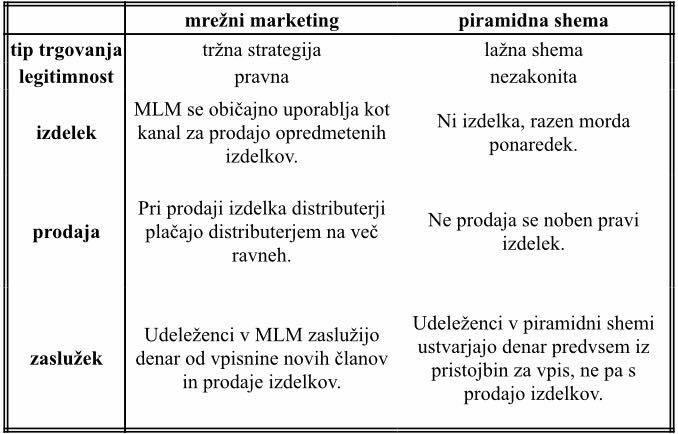
\includegraphics[height=5cm]{tab}\\

\subsection{Najodmevnejše goljufije}

\subsubsection{Ponzi}

Ponzijeva shema se imenuje po italijanskem priseljencu Charlesu Ponziju (1882-1949) v ZDA. Ponzi je bil karizmatični italijanski imigrant, ki je v letih okrog 1920 opeharil vlagatelje za približno 20 milijonov takratnih dolarjev, kar je toliko, kot je danes 215 milijonov dolarjev. Ponzi je vlagateljem obljubil petdesetodstotni donos v samo 45 dneh oziroma stoodstotni donos v samo 90 dneh. Trdil je, da je takšne donose možno ustvariti z odkupi kuponov za povratno pošto, ki so jih Američani s poštnimi pošiljkami pošiljali v tujino. Svojo pot je začel s takratnimi pet tisoč dolarji, dva meseca zatem jih je imel že 420 tisoč. Večina vlagateljev si ni izplačevala dobičkov, ampak je vse nalagala nazaj v shemo. Nekateri so celo jemali hipoteke na hišo, zato da bi bili del te »pravljice«. Na vrhu evforije je v samo treh urah zbral milijon dolarjev. Toda finančniki, ki so se čudili, kako Ponzi ustvarja takšne donose, so ga hitro razkrinkali. Da bi sistem deloval, bi moralo biti v obtoku 160 milijonov kuponov, a jih je bilo le 27 tisoč. Na ameriški pošti so dejali, da takšna količina ni bila kupljena ne v ZDA ne v tujini. Ljudi je zagrabila panika. Ponzi je samo v prvih treh dneh izplačal dva milijona dolarjev, torej skoraj desetino vplačil. V pol leta od začetka prevare je bil Ponzi insolventen in je imel približno sedem milijonov dolarjev dolgov, ki niso bili nikoli poplačani. Poleg Ponzija pa je bankrotiralo tudi pet bank. Zaradi goljufije in kraje je odsedel le 12 let in pol, po izpustu iz zapora so ga deportirali v Italijo. Tam se je celo zaposlil v finančnem oddelku italijanske vlade Benita Mussolinija in tudi njega prinesel okoli, zato je moral zbežati v Južno Ameriko, kjer pri 66 letih v revščini umrl.
Ponzi pa ni idejni oče teh prevar, saj naj bi model, ki ga je uporabil, nastal kar 120 let pred njim. Izumil ga je William Miller, katerega goljufija je bila vredna milijon dolarjev (današnjih 25 milijonov dolarjev), svojim vlagateljem pa je obljubljal kar 520-odstotne letne donose. Ko je bil razkrinkan, je šel za 10 let v zapor.

\subsubsection{Marconi}
Leta 2013 je bil na 12 let zapora obsojen Nello Marconi, lastnik družbe Remius, ki je osnoval največjo finančno piramido pri nas. Priznal je krivdo za 140 dejanj poslovne goljufije in pranja denarja. Vlagatelje je zavajal, da bo njihove vložke plemenitil na valutnem trgu forex in jim izplačeval 10-odstotne donose na mesec. Po ocenah naj bi dolgoval vsaj 20 milijonov evrov. Kje je ta denar, pa je tudi sam Marconi, priznal, da ne ve.

\subsubsection{Madoff}
Največjo prevaro utemeljeno na delovanju Ponzijeve sheme je izvedel Bernard Madoff, znan in spoštovan borzni posrednik, ustanovitelj podjetja za trgovanje z vrednostnimi papirji, ki je pozneje nosilo njegovo ime - Bernard L. Madoff Investment Securities. Veljal je za odličnega strokovnjaka za delniške trge, njegovo ime in njegov sloves sta imela dovolj veliko težo, da sta privabljala stranke. V zgodnjih devetdesetih letih je postal tudi predsednik nadzornega sveta ameriške borze Nasdaq.
To bi moralo biti dovolj, da bi ga na Wall Streetu še dolgo imeli v dobrem spominu. A se ga bodo spominjali po čisto drugih rečeh. Seznam tistih, ki jih je oškodoval, je namreč zelo zelo dolg. Sega od dobrodelnih ustanov do zasebnih vlagateljev v New Yorku in na Floridi – v središču škandala je bil Palm Beach Country Club, ekskluzivni golf klub, kjer je Madoff rekrutiral veliko zasebnih vlagateljev. Prizadetih je tudi precej evropskih bank: španskih, britanskih, francoskih (Natixis 554 mio), avstrijskih (Medici 2,1 mrd), nemških (Allianz, Volksbank, Raiffeisenbank) in švicarskih.
Tekmeci so domnevali, da Madoff pač izrablja informacije o velikih nakupih in prodajah delnic, ki vplivajo na gibanje tečajev, v svojo korist. Navedbe o njegovi naložbeni strategiji so bile vedno nejasne, vlagatelje pa je zavajal z rednimi in podrobnimi poročili o transakcijah, ki pa so bile verjetno izmišljene.
Skrivnost Madoffove prepričljivosti so bile zmerne obljube. Značilno je, da goljufi, ki delujejo po Ponzijevem sistemu, obljubljajo zelo visoke donose. Madoff pa je obljubljal 10- do 15-odstotni donos na leto, kar je bilo videti povsem realistično. Kljub nestanovitnim borzam pa je bila nenavadna dolgoletna stalnost dobičkov. Ravno zaradi domnevno konservativne naložbene strategije je Madoff pridobival zaupanje vlagateljev. Da vodi sistem, ki mu nekateri pravijo tudi piramidni, si ni mislil skoraj nihče.
Madoff je v vsaj 20 letih delovanja svoje vlagatelje ogoljufal za kar 65 milijard ameriških dolarjev. Razkrit je bil, ko zaradi finančne krize ni mogel izplačati nekaterih vlagateljev, ki so zahtevali umik svojega denarja. Leta 2009 je priznal zločine in bil za prevaro obsojen na 150 let zapora, vse njegovo premoženje pa so zaplenili in prodali na dražbi, za poplačilo prevaranih vlagateljev.


\section{Zaključek}

Spoznali smo osnovne pojme decentralizacije, ki smo jih aplicirali na prepoznavne sisteme, ki ta koncept uporabljajo. Z analizo delovanja ideje na primeru blockchain tehnologije smo podrobno spoznali funkcije, ki jih ta opravlja, in katere probleme reši. Razvidna je velika vloga tega sistema v podjetjih, kot sta Ripple in Ethereum, ki ga uporabljajo za več namenov in ne samo kot transakcijski izkaz. Videli smo pomembnost kriptovalut kot korak v smeri razvoja proti decentralizaciji. Po pregledu klasične monetarne politike smo opazili prednosti novih sistemov, kot so preprečitev umetne inflacije, večja pretočnost trga, preprostejše prenašanje denarja,…  Pregledali smo prednosti in slabosti ICO in videli njihovo uporabno vrednost za ustvarjalce in kaj pomeni za investitorje. Raziskali smo tudi zlorabe kriptovalut, ločene od tega. Po vsem tem lahko rečemo, da imajo kriptovalute prihodnost, čeprav svet in kriptovalute same še niso nujno pripravljene, da popolnoma nadomestijo klasične denarne valute. Njihova stabilnost se namreč zanaša predvsem na uporabnike, zaradi česar je njihova hramba lahko tvegana, predvsem v primeru nepoznavanja sistema.

\begin{thebibliography}{9}

\bibitem{} 
Coindesk. (2019). Bitcoin (EUR) Price. Pridobljeno 8. maj 2019 iz
\\\texttt{https://www.coindesk.com/price/bitcoin}

\bibitem{} 
Buttice, C. (2018). Are Cryptocurrencies the True Future of the World's Economy? Pridobljeno 5. maj 2019 iz
\\\texttt{https://www.techopedia.com/are-cryptocurrencies-the-true-future-of-the-worlds-economy/2/33480}

%\bibitem{} 
%Litvack, J. (2007). What is Decentralization? Pridobljeno 26. april 2019 iz
%\\\texttt{http://www.ciesin.org/decentralization/English/General/Different_forms.html}

\bibitem{} 
Canellis, D. (2018). Here’s how criminals use Bitcoin to launder dirty money. Pridobljeno 2. maj 2019 iz
\\\texttt{https://thenextweb.com/hardfork/2018/11/26/bitcoin-money-laundering-2/}

%\bibitem{} 
%Bonnal, J. (2007). A History of Decentralization. Pridobljeno 6. maj 2019 iz
%\\\texttt{http://www.ciesin.org/decentralization/English/General/history_fao.html}

\bibitem{} 
DeMartino, I. (2014). Top 5 Moments In Decentralization History. Pridobljeno 8. maj 2019 iz
\\\texttt{https://cointelegraph.com/news/top-5-moments-in-decentralization-history}

\bibitem{} 
The World Bank Group. (2001). Administrative Decentralization. Pridobljeno 5. maj 2019
\\\texttt{http://www1.worldbank.org/publicsector/decentralization/admin.html}

\bibitem{} 
Miller, K. (2002). Advantages and disadvantages of local government decentralization. Pridobljeno 30. april 2019
\\\texttt{https://pdfs.semanticscholar.org/5e82/ec8b21d7e3673ec1b195430a24743e748b62.pdf}

\bibitem
Sylla, R., Wright, R. E., and Cowen, D. J. (2009). Alexander Hamilton, Central Banker: Crisis Management During the US Financial Panic of 1792. Business History Review, 83(01), 61-86. 

%\bibitem{} 
%Brezovnik, B. (2008). Decentralizacija v teoriji in praksi. Pridobljeno 5. maj 2019 iz
%\\\texttt{http://www.lex-localis.info/files/14573914-cb5f-4c22-8bc1-280c0a26bee9/633415636460000000_lex%20localis_1-2008_pp.%2087-103,%20brezovnik.pdf?fbclid=IwAR1bR-0nSZDxsIiTjcDxh8xv5mZimOcp6yuQgy-_oSljdrAJEGA4NHmEXhM}

%\bibitem{} 
%Palitha. (2017). Decentralization bitcoin's Achilles' heel. Pridobljeno 4. maj 2019 iz
%\\\texttt{http://www.chinadaily.com.cn/opinion/2017-08/15/content_30623588.html}

%\bibitem{} 
%Dancheva, O. (2014). Decentralization: how public opinion changes. Pridobljeno 8. maj 2019 iz
%\\\texttt{http://despro.org.ua/upload/medialibrary/%D0%B1%D1%83%D0%BA%D0%BB%D0%B5%D1%82%20%D0%A4%D0%BE%D0%BA%D1%83%D1%81-%D0%93%D1%80%D1%83%D0%BF%D0%BF%D1%8B_eng_2.pdf}

\bibitem{} 
Kistler, S. (2014). 20th-century centralization and 21st-century decentralization. Pridobljeno 8. maj 2019 iz
\\\texttt{https://temporachristiana.wordpress.com/2014/09/30/20th-century-centralization-and-21st-century-decentralization/}

\bibitem{} 
Freemansperspective. (2016). Centralization vs. Decentralization. Pridobljeno 3. maj 2019 iz
\\\texttt{https://www.freemansperspective.com/centralization-vs-decentralization/}

\bibitem{} 
Tsihitas, T. (2017). Ripple vs Bitcoin Comparison. Pridobljeno 27. april 2019 iz
\\\texttt{https://coincentral.com/ripple-vs-bitcoin/}

\bibitem{} 
Ripple. (2019). Pridobljeno 28. april 2019 iz
\\\texttt{ https://ripple.com/}

\bibitem{} 
Cointelegraph. (2019). Ripple Vs. Bitcoin: Key Differences. Pridobljeno 2. maj 2019 iz
\\\texttt{https://cointelegraph.com/ripple-101/ripple-vs-bitcoin-key-differences}

\bibitem{} 
CoinCodex. (2019). Ripple Price Index. Pridobljeno 2. maj 2019 iz
\\\texttt{https://coincodex.com/crypto/ripple/}

%\bibitem{} 
%Bitcoin Wiki. (2017). Value overflow incident. Pridobljeno 7. maj 2019 iz
%\\\texttt{https://en.bitcoinwiki.org/wiki/Value_overflow_incident}

%\bibitem{} 
%Jimi S. (2018). How does blockchain work in 7 steps — A clear and simple explanation. Pridobljeno 4. maj 2019 iz
%\\\texttt{https://blog.goodaudience.com/blockchain-for-beginners-what-is-blockchain-519db8c6677a}

%\bibitem{} 
%Kenton, W. (2018). Decentralized market. Pridobljeno 7. maj 2019 iz
%\\\texttt{https://www.investopedia.com/terms/d/decentralizedmarket.asp}

%\bibitem{} 
%Shavit, D. (2019). A History of Decentralized Thought. Pridobljeno 2. maj 2019 iz
%\\\texttt{https://www.youtube.com/watch?v=IXTpGq85RB4&feature=youtu.be&fbclid=IwAR0zjJVnrF4VAZv4CMuEixJ_JAbAogUeWk4X_AR9qTE2w7KUtIkVR8lY-9A}




\end{thebibliography}

\end{document}